\documentclass{standalone}
\usepackage[T1]{fontenc}
\usepackage[latin2]{inputenc}
\usepackage[english]{babel}
\usepackage{tikz}
\usepackage{times}
\usetikzlibrary{calc,through,backgrounds,positioning,fit}
\usetikzlibrary{shapes,arrows,shadows,calendar}
\begin{document}
 
\centering

\begin{tikzpicture}
\node (A)[label={State graph}] at (3,0) {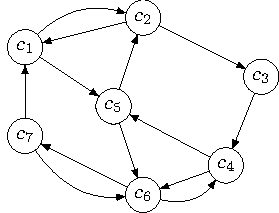
\includegraphics[scale=1]{statesgraph.pdf}};
\node (B)[label={Data with cluster assigned}]  at (-5,0) {
\begin{tabular}{|c|c|c|c|c|c||c|}
\hline
\(t\) & \(a_1\) & \(a_2\)  &\(a_3\)  &\dots &\(a_k\) &\(c\) \\
\hline\hline
\(t_1\) & \(v^1_1\) & \(v^1_2\) & \(v^1_3\) & \dots & \(v^1_k\) &\(c_1\) \\ \hline
\(t_2\) & \(v^2_1\) & \(v^2_2\) & \(v^2_3\) & \dots & \(v^2_k\) &\(c_2\) \\ \hline
\dots   & \dots     & \dots     & \dots     & \dots & \dots     &\dots   \\ \hline
\(t_n\) & \(v^n_1\) & \(v^n_2\) & \(v^n_3\) & \dots & \(v^n_k\) &\(c_n\) \\ \hline
\dots   & \dots     & \dots     & \dots     & \dots & \dots     &\dots   \\ \hline
\end{tabular}
};

\draw[draw=lightgray,->,line width=1mm] (B) --(A) node[midway,above,text width=15mm]{
Process discovery};

\end{tikzpicture}

\end{document}